%
%	Praxisbezug
%

\pagebreak
\section{CIS Scans}

\onehalfspacing

\subsection{CIS Benchmarks for Kubernetes}

In the previous chapter we've covered the basic mechanism to codify and enforce standards for our Kubernetai across the IT organization using Terraform and Rancher templates.

There are many security standards and recommendations available, but there is one organization that's universally recognized as leading the field of IT security and compliance: The Center for Internet Security, Inc. (CIS®)

CIS is a community-driven nonprofit and responsible for CIS Controls® and CIS Benchmarks™, which are globally recognized as the best practices for securing IT systems and data. If you want to have a look at the actual CIS Benchmarks, they are available for download on the CIS website, but you'll need to register with CIS first.

Testing a platform against a CIS Benchmark is a lengthy process. Fortunately there are a number of automated scans available for Kubernetes, and with Rancher 2.4 a CIS Scan is available for all managed Clusters right from the Rancher GUI.

CIS Scans can be invoked manually or scheduled on a regular basis. With Provider 1.8.0 (March 2020), this feature is now also available in Terraform.\footnote{See \textit{Rancher Labs (2020)}: Changelog. \cite{ChangeLog}}

\subsection{CIS Scan GUI}

At the cluster level, Rancher offers two choices of CIS Scans:

\begin{itemize}
\item RKE-CIS-1.4 Permissive
\item RKE-CIS-1.4 Hardened
\end{itemize}

Both scans are based on the Kubernetes CIS Benchmark version 1.4, with a different set of controls and are adapted by Rancher to the underlying RKE. To pass the hardened profile, you'll need to fully adhere to the Rancher 2.3 Hardening guide.\footnote{See \textit{Rancher Labs (2019)}: Hardening Guide. \cite{hardeningGuide}}

The cluster we created in the previous chapter is using mostly default values and does not pass the scan with the hardened profile:

\begin{figure}[H]
\centering
\caption {CIS Scan GUI}
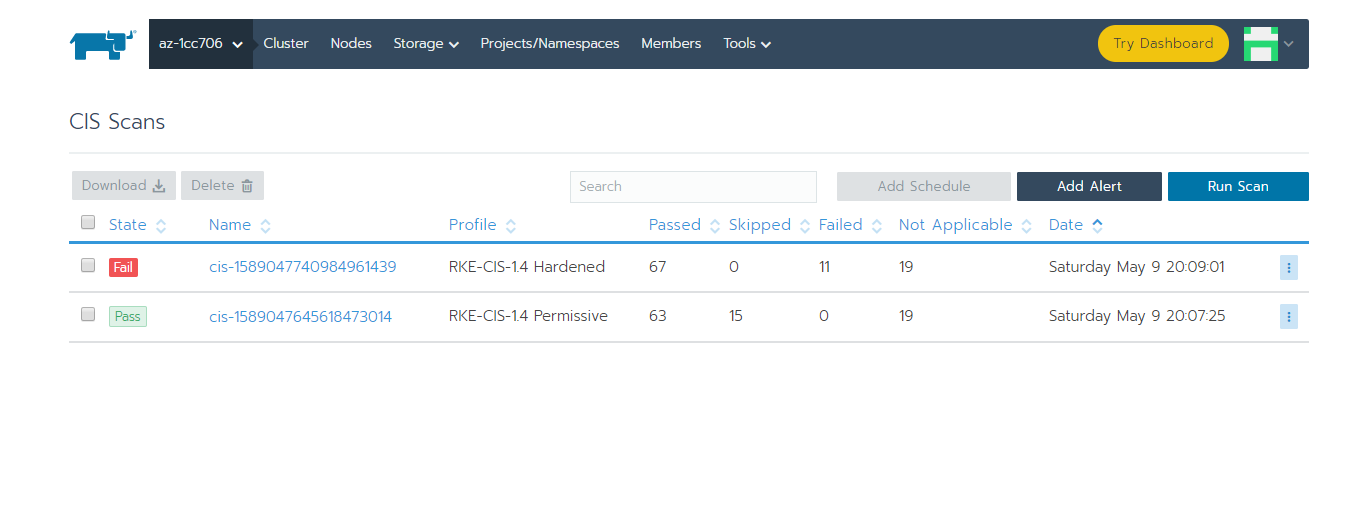
\includegraphics[width=\linewidth]{images/cis-scan-overview.png}
\label{fig:cisScanOverview}
\end{figure}

\subsection{Hardened CIS Scan}

We will not go through all hardening steps in detail, but use one control as an example:

\begin{figure}[H]
\centering
\caption {Hardened CIS Scan}
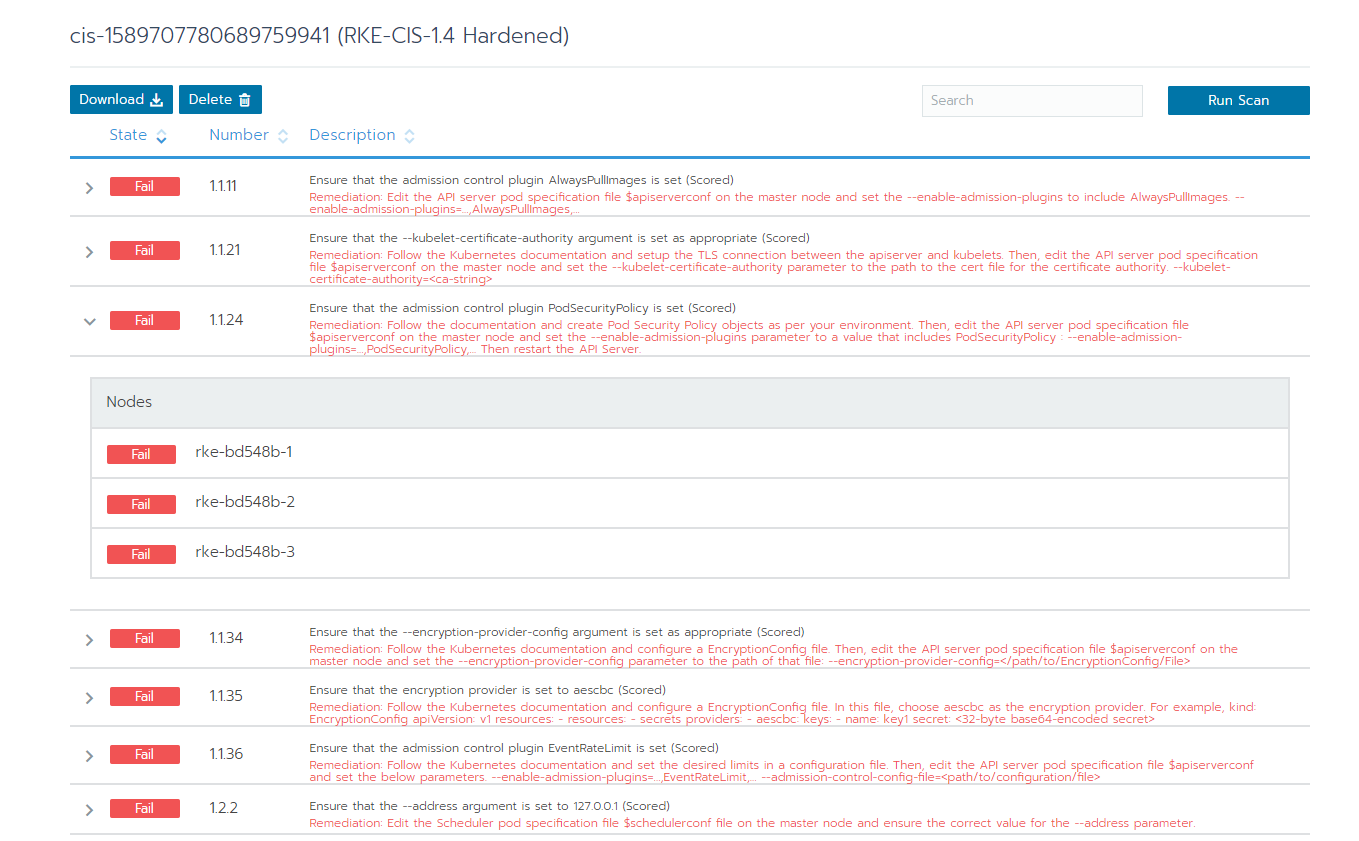
\includegraphics[width=\linewidth]{images/cis-scan-fail.png}
\label{fig:cisScanFail}
\end{figure}

The control we'll be focusing on is 1.1.24: Ensure that the admission control plugin PodSecurityPolicy is set.

To fully harden your cluster, please follow the hardening mentioned above.

\subsection{Kubernetes Security Policies}

What is a Pod Security Policy? Kubernetes provides two types of security policies, one for pod security and one for network security. Pod security policies, as the name implies, govern security-relevant aspects of pod specification,\footnote{See \textit{The Linux Foundation (2019)}: Pod Security Policies. \cite{podSecurity}} whereas network policies govern the allowed communication between groups of pods and the outside world.\footnote{See \textit{The Linux Foundation (2019)}: Network Policies. \cite{netSecurity}}

It is good practice when running a Kubernetes cluster in production to secure access with Pod Security Policies.\footnote{See \textit{Price, J. (2020)}: Kubernetes - Pod Security Policies. \cite{examplePsp}} Rancher offers pre-built PSPs (named "restricted" and "unrestriced") and a GUI to create your own.\footnote{See \textit{Iradier, A. (2020)}: Enhancing Kubernetes Security with Pod Security Policies. \cite{detailPsp}}

There are many controls within a Pod Security Policy that we won't be able to cover in this document, instead we'll focus on one an example.

\subsection{Remediation}

The scan gives us the following remediation details:

\verb|Remediation: Follow the documentation and create Pod Security Policy objects as per your environment|

To mitigate the failed control, what we need to do is to add a default Pod Security Policy. Fortunately, that's fairly easy in Rancher. In the cluster template we need to enable PSP support and define the default policy.

We can do that by adding the following line to our template definition in Terraform:

\begin{lstlisting}[caption=Cluster Template, frame=single, basicstyle=\ttfamily]
default_pod_security_policy_template_id = "restricted"
\end{lstlisting}

Or, if your prefer the Rancher GUI, you can set the default Pod Security Policy there too:

\begin{figure}[H]
\centering
\caption {Rancher PSP Support}
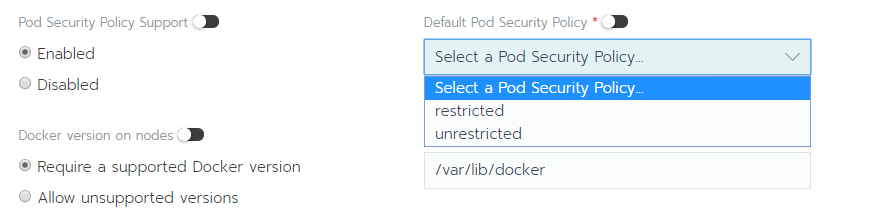
\includegraphics[width=\linewidth]{images/rancher-psp-support.png}
\label{fig:rancherPSP}
\end{figure}

Based on the needs of your IT organisation, you'll have to identify the critical controls and implement the remediation steps as needed, to harden your cluster.

Automated CIS scans give you a very valuable tool to regularly check all your Kubernetai for security issues and regulatory compliance and act on issues accordingly.
